\documentclass[10pt]{standalone}
\usepackage{pgfplots}
\pgfplotsset{compat=1.15}
\usepackage{mathrsfs}
\usetikzlibrary{arrows}
\pagestyle{empty}
\begin{document}
\definecolor{ccqqqq}{rgb}{0.8,0,0}
\definecolor{qqwuqq}{rgb}{0,0.39215686274509803,0}
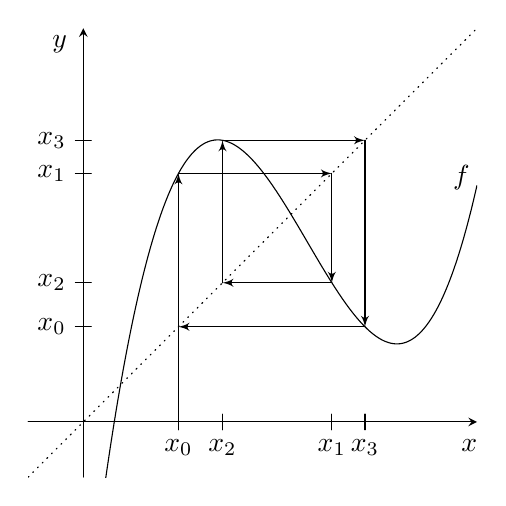
\begin{tikzpicture}[line cap=round,line join=round,>=triangle 45,x=1cm,y=1cm]
\begin{axis}[
x=1cm,y=1cm,
axis lines=middle,
grid style=dashed,
xmin=-0.7,
xmax=5,
ymin=-0.7,
ymax=5,
xtick={0},
ytick={0},
%xtick={-1,0,...,5},
%ytick={0,1,...,4},
]
\clip(-1,-0.7) rectangle (5,5);
\draw[smooth,samples=100,domain=-1:5] plot(\x,{0.4393529422369385*(\x)^(3)-3.748727793458679*(\x)^(2)+8.954313779825904*(\x)-2.9649021143619496});
\draw[ dotted,smooth,samples=3,domain=-1:5.5] plot(\x,{(\x)});


\draw[-latex'] (1.208,0)-- (1.208,3.1560127906097932);
\draw[-latex'] (1.208,3.1560127906097932)-- (3.1560127906097932,3.1560127906097932);
\draw[latex'-] (3.1560127906097932,1.767284417093526)-- (3.1560127906097932,3.1560127906097932);
\draw[-latex'] (3.1560127906097932,1.767284417093526)-- (1.767284417093526,1.767284417093526);
\draw[latex'-] (1.767284417093526,3.576655325498841)-- (1.767284417093526,1.767284417093526);
\draw[-latex'] (1.767284417093526,3.576655325498841)-- (3.576655325498841,3.576655325498841);
\draw[latex'-] (3.576655325498841,1.2083856388070355)-- (3.576655325498841,3.576655325498841);
\draw[-latex'] (3.576655325498841,1.2083856388070355)-- (1.2083856388070355,1.2083856388070355);

\draw (1.208,0.1) -- (1.208,-0.1) node[below] {$x_0$};
\draw (3.1560127906097932,0.1) -- (3.1560127906097932,-0.1) node[below] {$x_1$};
\draw (1.767284417093526,0.1) -- (1.767284417093526,-0.1) node[below] {$x_2$};
\draw (3.576655325498841,0.1) -- (3.576655325498841,-0.1) node[below] {$x_3$};

\draw (0.1,1.208) -- (-0.1,1.208) node[left] {$x_0$};
\draw (0.1, 3.1560127906097932) -- (-0.1, 3.1560127906097932) node[left] {$x_1$};
\draw (0.1, 1.767284417093526) -- (-0.1, 1.767284417093526) node[left] {$x_2$};
\draw (0.1, 3.576655325498841) -- (-0.1, 3.576655325498841) node[left] {$x_3$};


\begin{scriptsize}
\draw (4.8,3.1) node {$f$};
\draw (4.9,-.3) node {$x$};
\draw (-.3,4.8) node {$y$};
\end{scriptsize}
\end{axis}
\end{tikzpicture}
\end{document}